\documentclass[10pt]{beamer}

\usetheme[progressbar=frametitle]{metropolis}
\usepackage{appendixnumberbeamer}
\usepackage{amsmath}
\usepackage[mathscr]{euscript}
\usepackage{booktabs}
\usepackage{rotating}
\usepackage[scale=2]{ccicons}
\DeclareMathOperator*{\argmax}{argmax}
\DeclareMathOperator*{\argmin}{argmin}
% Copied from mathrsfs.sty
\usepackage{multirow}
\DeclareSymbolFont{rsfs}{U}{rsfs}{m}{n}
\DeclareSymbolFontAlphabet{\mathscrsfs}{rsfs}
\usepackage{pgfplots}
\usepgfplotslibrary{dateplot}
\usepackage{graphicx}
\usepackage{subcaption}
\usepackage{xspace}
\newcommand{\themename}{\textbf{\textsc{metropolis}}\xspace}

\title{Virtual Shape Recognition using Leap Motion}
\subtitle{EC 520: Digital Image Processing and Communication}
% \date{\today}
\date{}
\author{Aditya Chechani and Harshil Prajapati}
\institute{Department of Electrical and Computer Engineering: Boston University}
% \titlegraphic{\hfill\includegraphics[height=1.5cm]{logo.pdf}}

\begin{document}

\maketitle

\begin{frame}[fragile]{Problem Statement}
  To develop a robust algorithm to extend Leap Motion capabilities to recognize hand drawn gestures of various 2D shapes (e.g. circle, ellipse, square, triangle, etc.)
  \begin{figure}
    \centering
    \begin{subfigure}[b]{0.35\textwidth}
        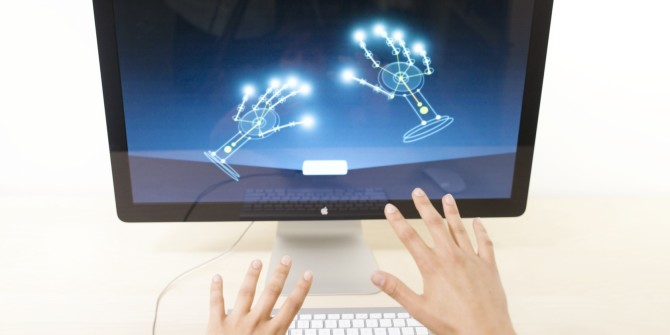
\includegraphics[width=\textwidth, height = 3cm]{leap}
        \caption{Leap Motion \cite{leap}}
    \end{subfigure}
    \begin{subfigure}[b]{0.5\textwidth}
        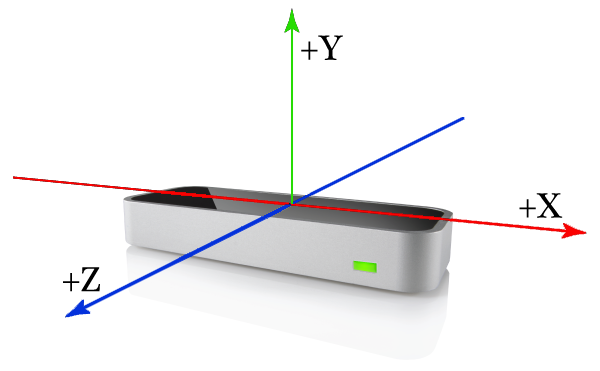
\includegraphics[width=\textwidth, height = 3cm]{Leap_Axes}
        \caption{Coordinates axes of Leap Motion }\label{fig:leapaxes}
    \end{subfigure}
\end{figure}
\end{frame}

\begin{frame}[fragile]{Data Acquisition }
\begin{itemize}
\item Leap Motion SDK - Python
\item x,y,z coordinates of the tip of the index finger
\item Store it in .json file
\end{itemize}
\begin{columns}
  \begin{column}{0.4\textwidth}
% Please add the following required packages to your document preamble:
% \usepackage{multirow}
\begin{figure}
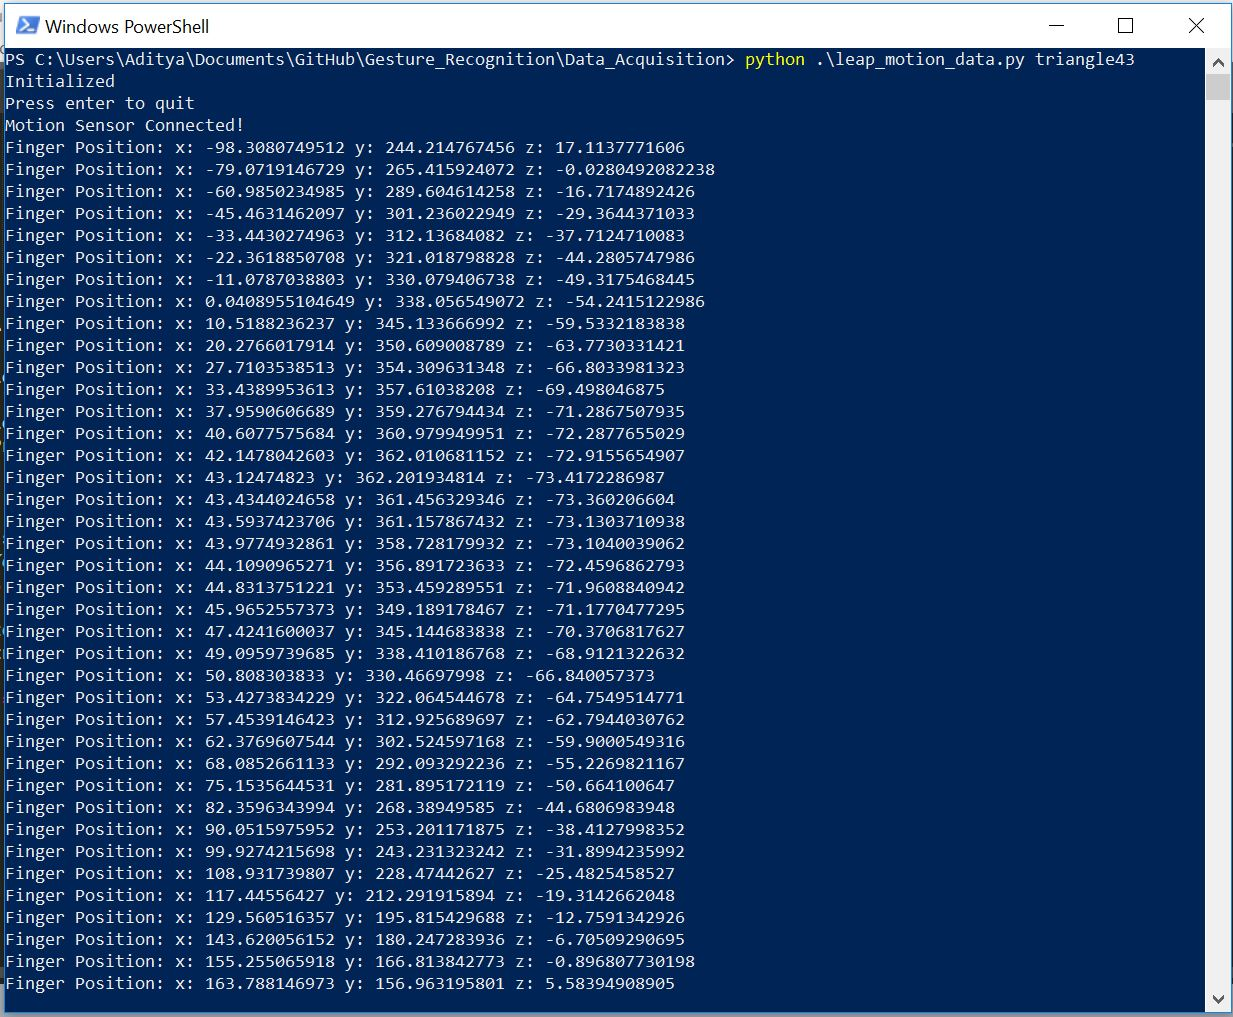
\includegraphics[width=\textwidth, height = 3cm]{data_acquisition}
\caption{Capturing Leap data}

\end{figure}
\end{column}
  \begin{column}{0.5\textwidth}  %%<--- here
 \begin{table}[]
\centering
\begin{tabular}{|l|l|}
\hline
\textbf{Shape }    & \textbf{Data} \\ \hline
Circle    & 50   \\ \hline
Rectangle & 50   \\ \hline
Triangle  & 50   \\ \hline
\end{tabular}
\caption{Generated Data}
\label{my-label}
\end{table}
  \end{column}
\end{columns}
\end{frame}


\begin{frame}{Data Preprocessing: \textit{Planner Fitting of 3D points} }
Shapes will not be on a plane $\parallel$ to XY plane of Leap Motion so we find a hypothetical plane z which has the least squared error with the data points provided \cite{eberly2000least}.

\begin{equation}
	z = A\textit{x} + B\textit{y} + D
\end{equation}
The coefficients of plane are given by 
\begin{equation*}
c_x = -\frac{A}{D};\hspace{15pt} c_y = - \frac{B}{D} ;\hspace{15pt} c_z = \frac{1}{D}
\end{equation*}
The normal vector of plane is 
\begin{equation}
n_p = [-\frac{A}{D} \hspace{10pt} -\frac{B}{D} \hspace{10pt} \frac{1}{D}] 
\end{equation}
Normal vector to X-Y plane 
\begin{equation*}
n_{XY} = [0\hspace{10pt}  0 \hspace{10pt}  1]
\end{equation*}
\end{frame}

\begin{frame}{Data Preprocessing: \textit{Planner Fitting of 3D points} }
Rotation Vector (u):
\begin{equation}
u = \frac{n_p}{\mid n_p \mid} \times n_{XY}
\end{equation}
Rotation angle ($\theta$):
\begin{equation}
\theta = sin^{-1} (\mid n_p \mid)
\end{equation}
Using the rotation vector and the angle we calculate rotation matrix "\textbf{R}" we get the transformed data
\begin{equation}
[x_{new},y_{new},z_{new}]^T  = R [x,y,z]^T
\end{equation}
\end{frame}

\begin{frame}{Data Preprocessing: \textit{Plane Fitting of 3D points} }
\begin{figure}
    \centering
    \begin{subfigure}[b]{0.4\textwidth}
        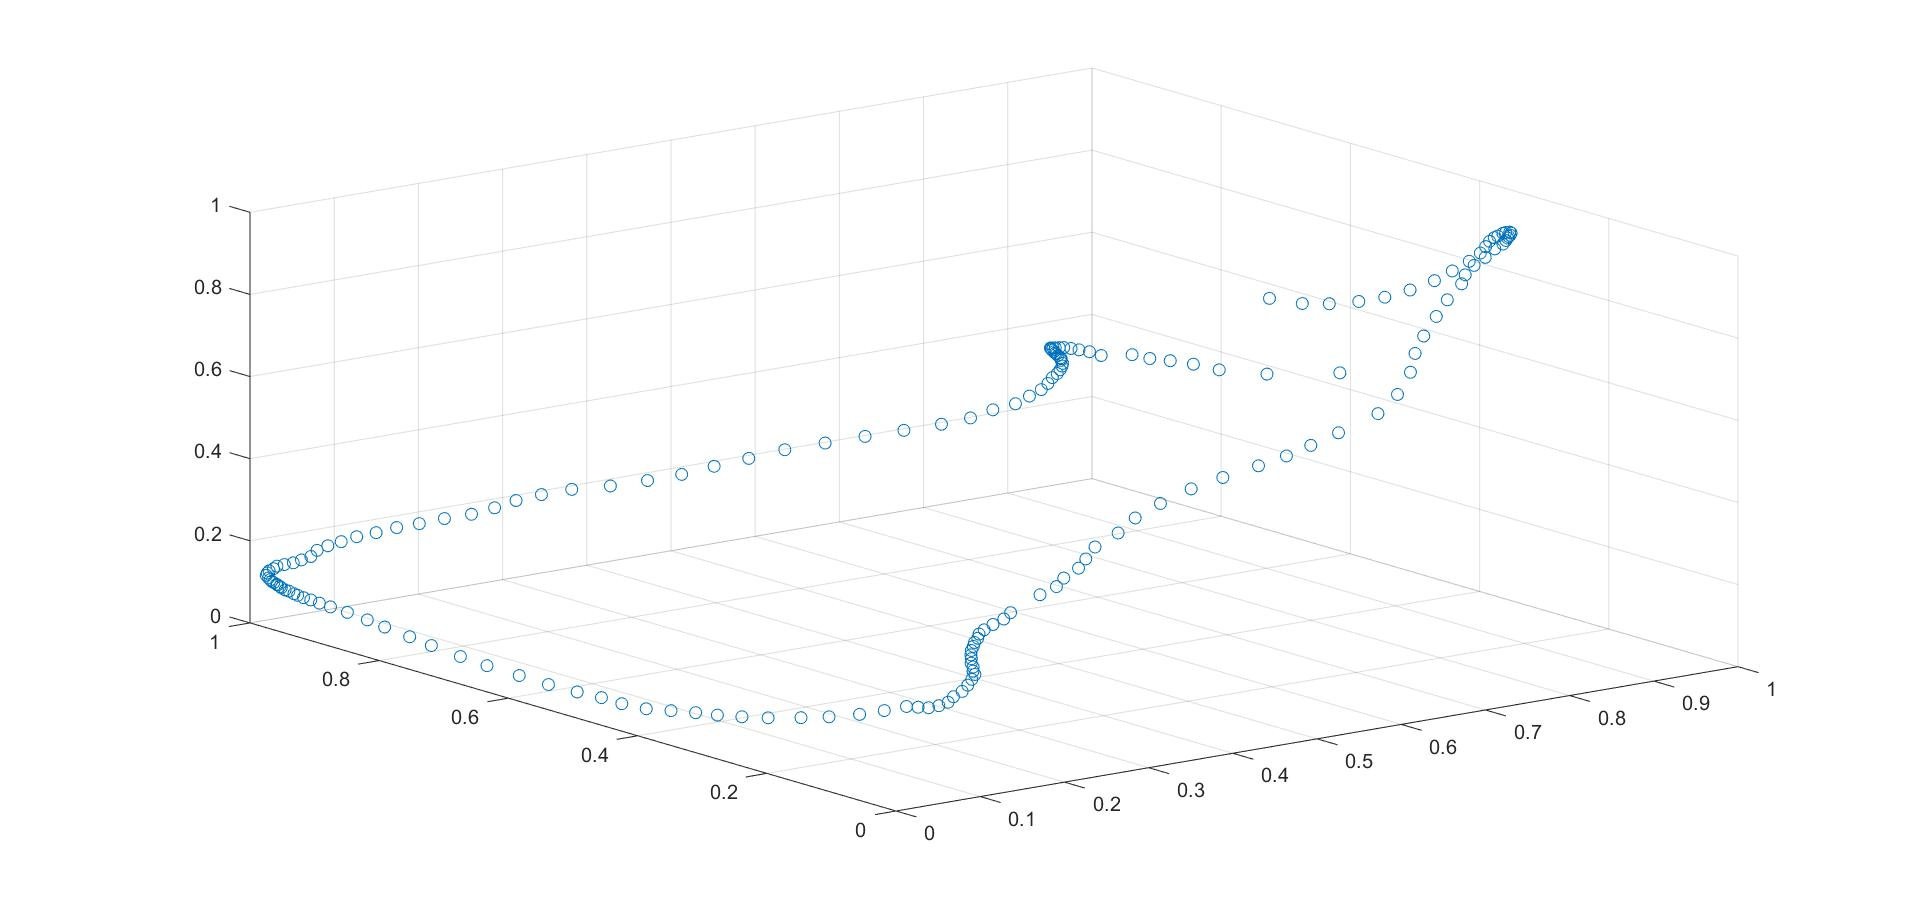
\includegraphics[width=\textwidth,height = 4cm]{scatter}
        \caption{Data points in 3D Space}
    \end{subfigure}
    \begin{subfigure}[b]{0.4\textwidth}
        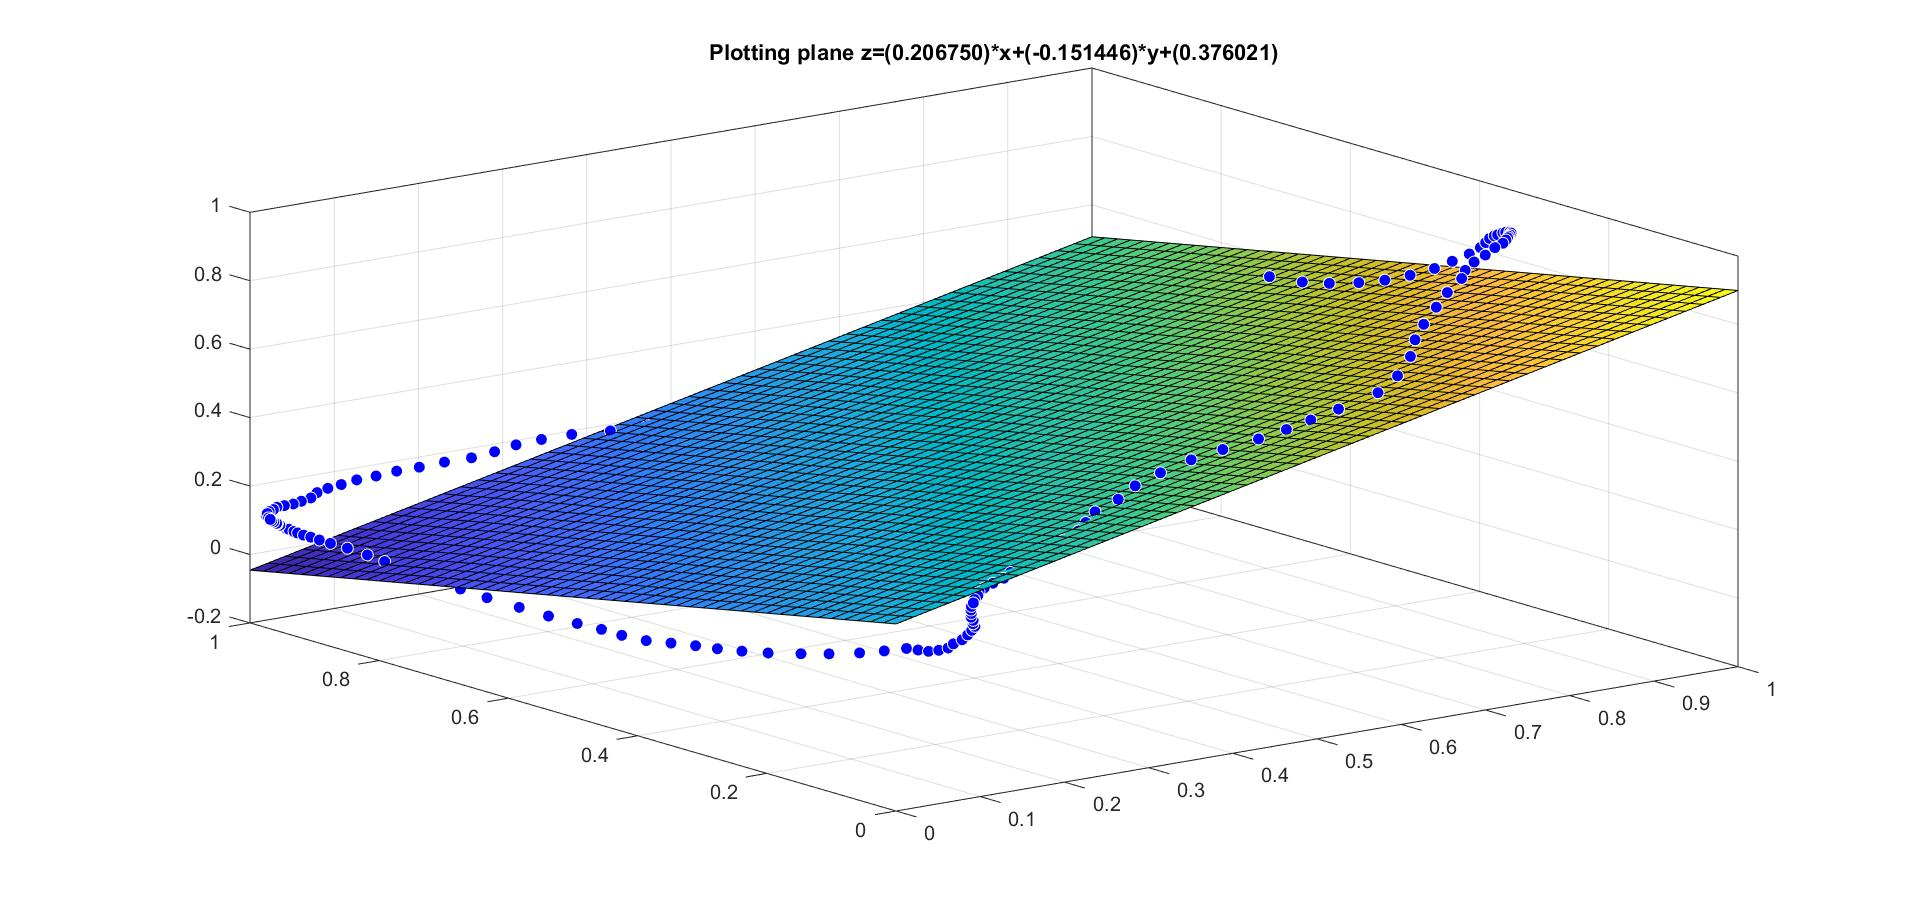
\includegraphics[width=\textwidth,height = 4cm]{plane_fit}
        \caption{Best Fitted Plane}
    \end{subfigure}
    \caption{Plane Fitting of 3D points}\label{fig:3dpts}
\end{figure}
\end{frame}

\begin{frame}{Data Preprocessing: \textit{Plane Fitting of 3D points} }
\begin{figure}
    \centering
    \begin{subfigure}[b]{0.4\textwidth}
        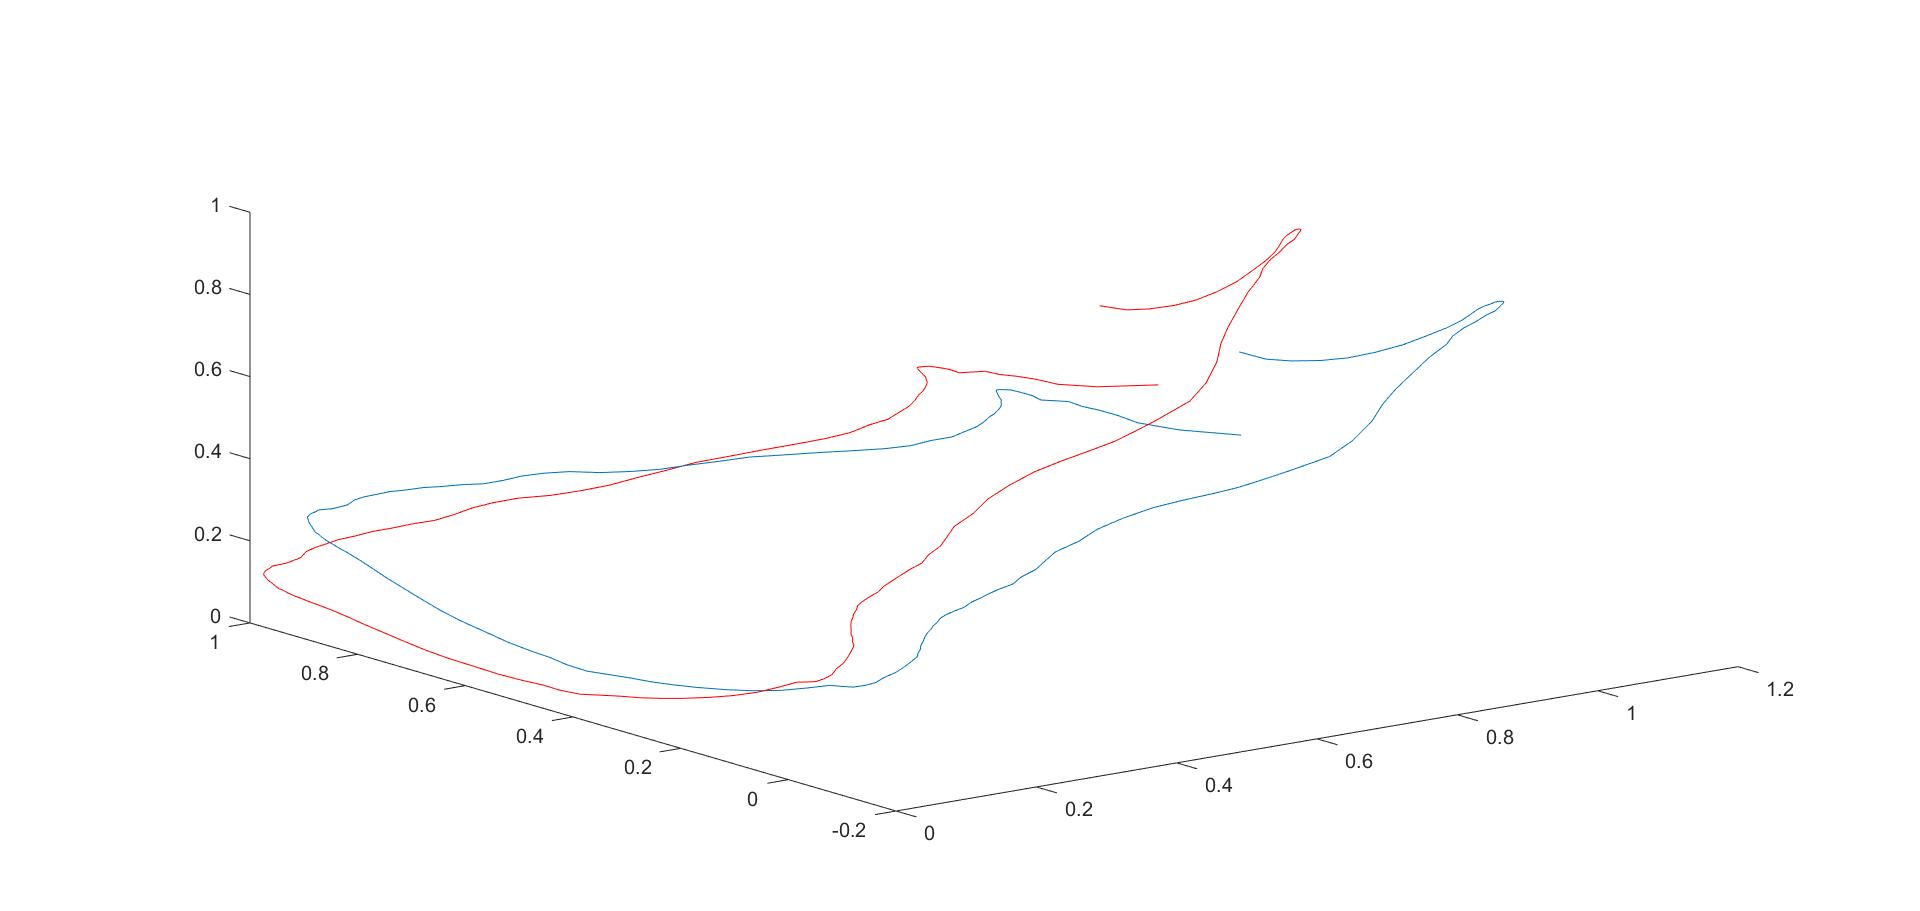
\includegraphics[width=\textwidth,height = 4cm]{rotated_3d_plot}
        \caption{Rotated coordinate in 3D space}
    \end{subfigure}
    \begin{subfigure}[b]{0.4\textwidth}
        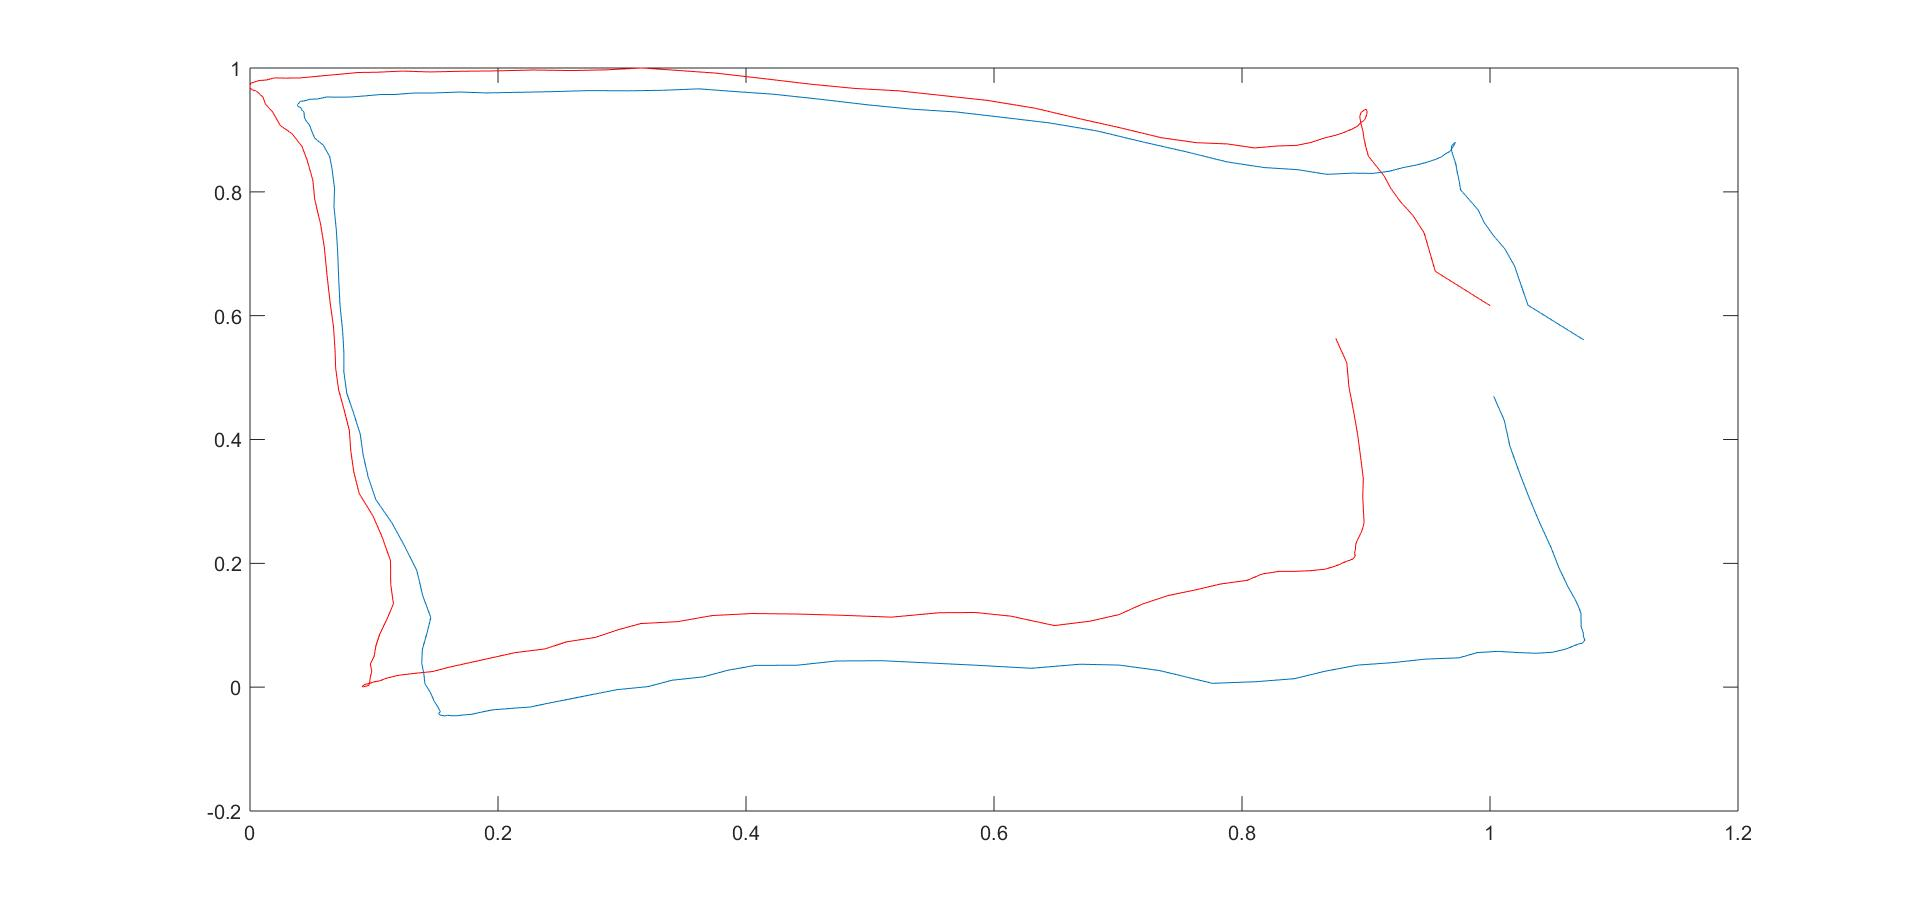
\includegraphics[width=\textwidth,height = 4cm]{rotated_2d_plot}
        \caption{Coodrinates on X-Y plane post processing}
    \end{subfigure}
    \caption{Plane Fitting of 3D points}\label{fig:3dpts}
\end{figure}
\end{frame}

\begin{frame}{Feature Extraction: \textit{Fourier Descriptor} }
Fourier Descriptor:
We define
\begin{equation*}
s[n] = x_n + iy_n
\end{equation*}
Taking the DFT of s[n]
\begin{equation}
a[k] = \frac{1}{N}\sum_{n=0}^{N-1}s[n]e^{\frac{-j2\pi n k}{N}}
\end{equation}
and coefficients can be recovered by 
\begin{equation}
s[n] = \sum_{k=0}^{N-1}a[k]e^{\frac{j2\pi n k}{N}}
\end{equation}
\end{frame}

\begin{frame}{Feature Extraction: \textit{Fourier Descriptor}}
\begin{figure}
    \centering
    \begin{subfigure}[b]{0.4\textwidth}
        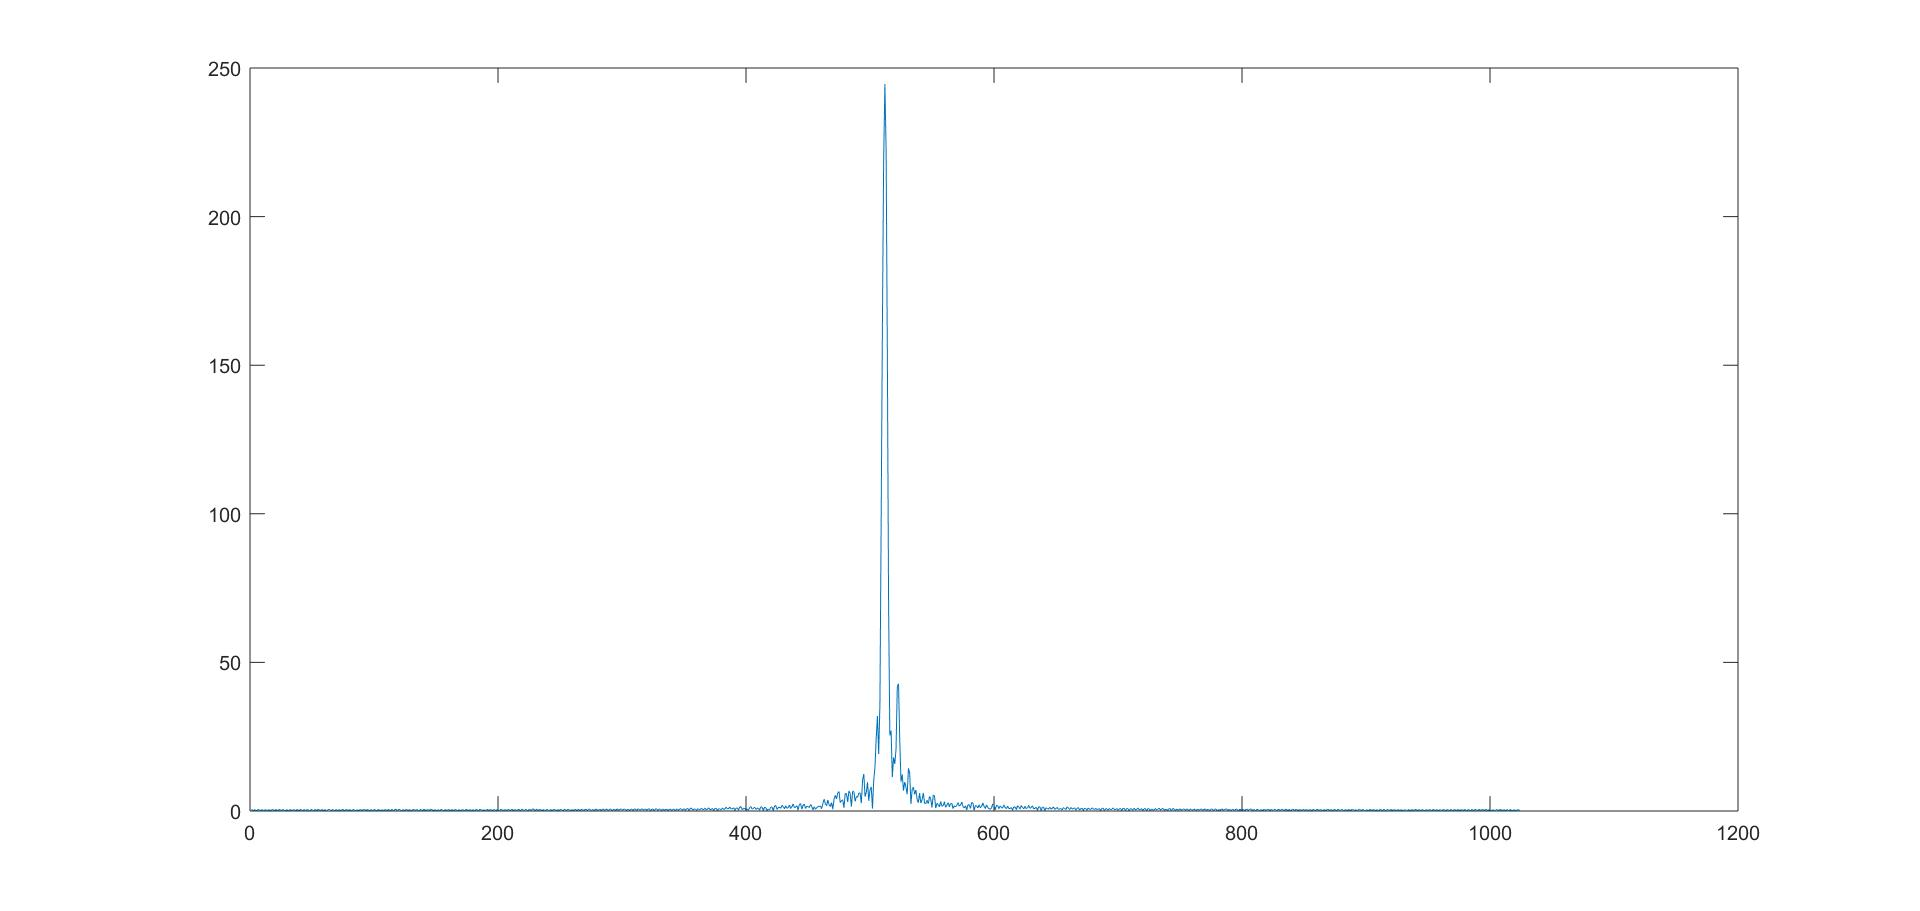
\includegraphics[width=\textwidth,height = 4cm]{shifted_fft}
        \caption{Fourier Descriptor of data points.}
    \end{subfigure}
    \begin{subfigure}[b]{0.4\textwidth}
        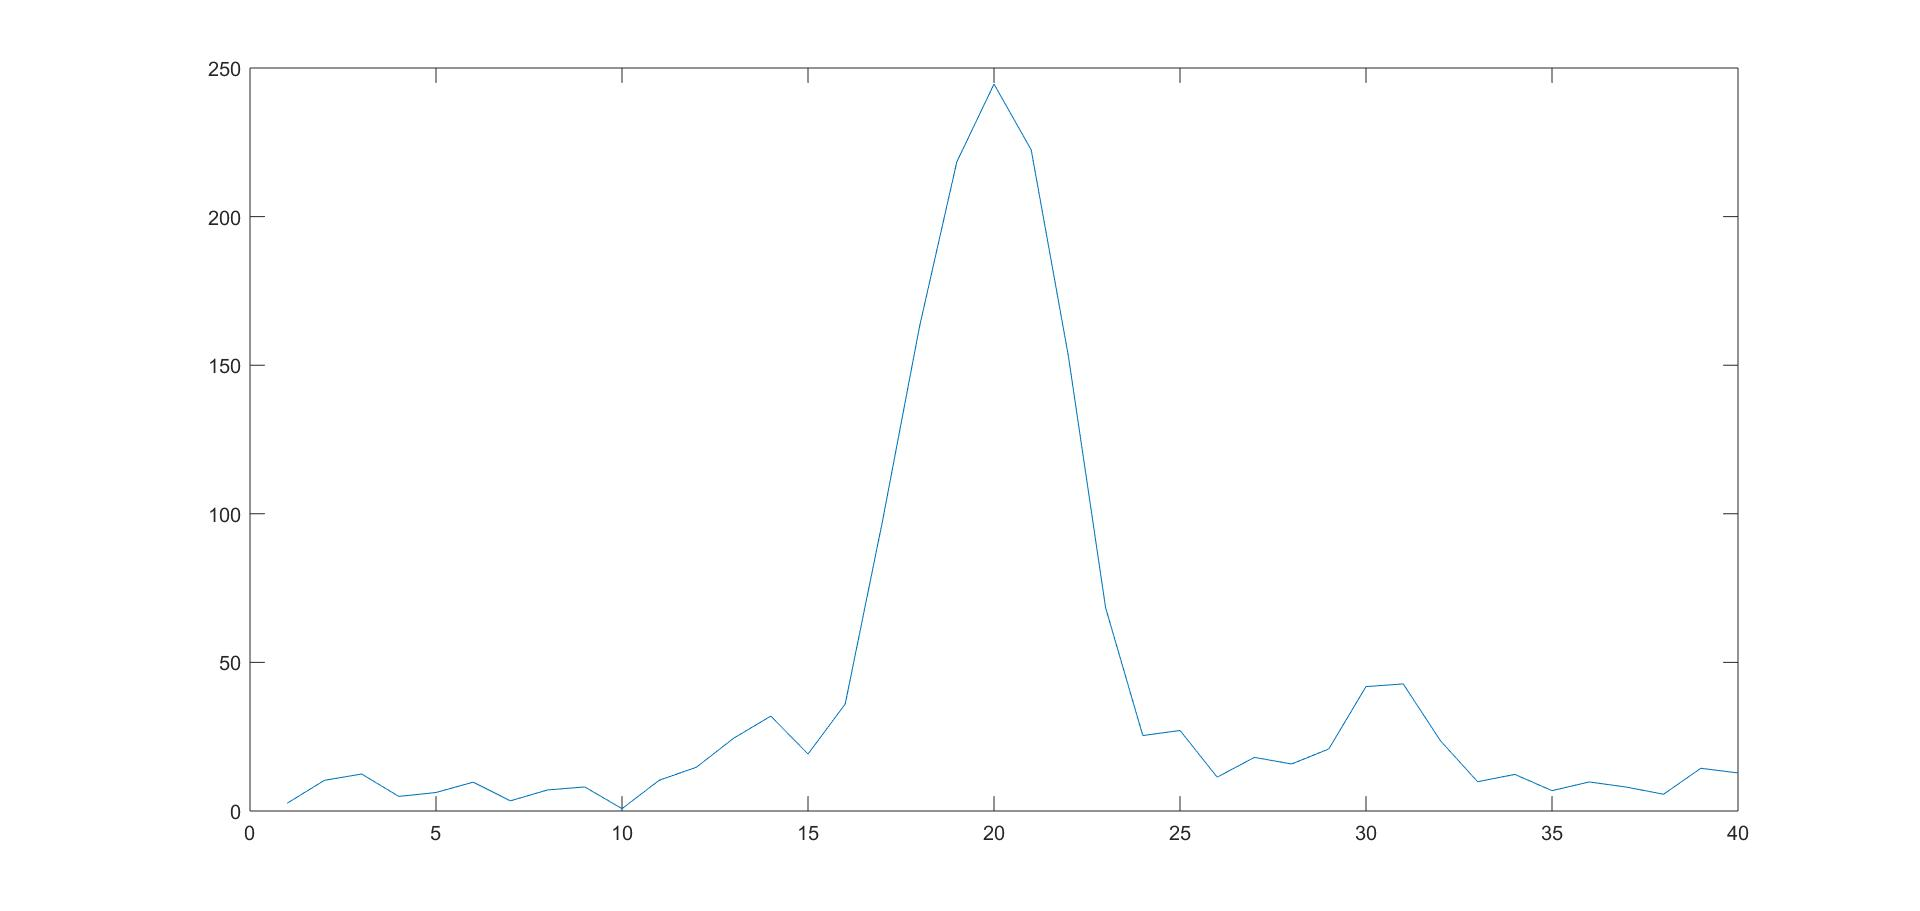
\includegraphics[width=\textwidth,height = 4cm]{shifted_fft_trimmed}
        \caption{Considering only 40 high energy points}
    \end{subfigure}
\end{figure}
\end{frame}

\begin{frame}{Classification: k-NN}
For a Data set $\mathscr{D} = {(\textbf{x}_1,y_1), \cdots (\textbf{x}_n,y_n)}$  with \textbf{x} as 20 point feature vector from feature extraction and test point \textbf{x}
Let ${(\textbf{x}_1,y_1), \cdots (\textbf{x}_n,y_n)}$  be reordered such that
\begin{equation*}
d(x,x_1) \leq d(x,x_2),\cdots d(x,x_n)
\end{equation*}
where $d(x,x_i) $ can be $l_p$ distance
\begin{equation*}
	\mid \mid x - x_{test} \mid \mid_p := (\sum_{i=1}^d \mid x_i - x_{test} \mid^p)^\frac{1}{p}
\end{equation*}
For our project we are considering the Euclidean distance ($l_2$)
\begin{equation}
h_{k-NN}  = \argmax_{y= 1 \cdot n} \sum^{k}_{j=1} 1(y_{(j)} = y)
\end{equation}
where $1(y_{(j)} = y)$   is the number of k-NNs of \textbf{x} with label =y \cite{ishwarspring18}\\
\end{frame}

\begin{frame}{Classification: k-NN}
\begin{figure}[h]
\centering
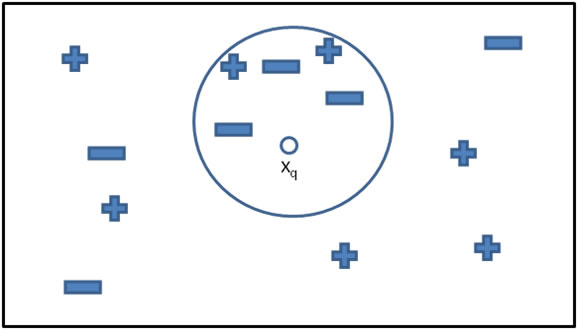
\includegraphics[width=\textwidth]{KNNExample}
\caption{k-NN Example \cite{knn}}
\end{figure}
\end{frame}

\begin{frame}{Classification: k-NN}
\begin{columns}
  \begin{column}{0.5\textwidth}
  
% Please add the following required packages to your document preamble:
% \usepackage{multirow}
\begin{table}[]
\centering
\begin{tabular}{l|l|l|l|}
\cline{2-4}
                                                                  & \multicolumn{3}{l|}{\textbf{Ground Truth}} \\ \hline
\multicolumn{1}{|l|}{\multirow{3}{*}{\rotatebox{90}{\textbf{Predict}}}} & 10         & 0         & 0        \\ \cline{2-4} 
\multicolumn{1}{|l|}{}                                            & 0          & 9         & 3        \\ \cline{2-4} 
\multicolumn{1}{|l|}{}                                            & 0          & 1         & 7        \\ \hline
\end{tabular}
\caption{80:20 Split (NN)}
\label{my-label}
\end{table}
\vspace{-20pt}
\centering CCR: 86.67\%
  \end{column}
  \begin{column}{0.5\textwidth}  %%<--- here
% Please add the following required packages to your document preamble:
% \usepackage{multirow}
\begin{table}[]
\centering
\begin{tabular}{l|l|l|l|}
\cline{2-4}
                                                                  & \multicolumn{3}{l|}{\textbf{Ground Truth}} \\ \hline
\multicolumn{1}{|l|}{\multirow{3}{*}{\rotatebox{90}{\textbf{Predict}}}} & 19        & 1         & 1         \\ \cline{2-4} 
\multicolumn{1}{|l|}{}                                            & 1         & 18        & 3         \\ \cline{2-4} 
\multicolumn{1}{|l|}{}                                            & 0         & 1         & 16        \\ \hline
\end{tabular}
\caption{60:40 Split (NN)}
\label{my-label}
\end{table}
\vspace{-20pt}
  \centering CCR: 88.33\%
  \end{column}
\end{columns}
\begin{columns}
  \begin{column}{0.5\textwidth}

% Please add the following required packages to your document preamble:
% \usepackage{multirow}
\begin{table}[]
\centering
\begin{tabular}{l|l|l|l|}
\cline{2-4}
                                                                  & \multicolumn{3}{l|}{\textbf{Ground Truth}} \\ \hline
\multicolumn{1}{|l|}{\multirow{3}{*}{\rotatebox{90}{\textbf{Predict}}}} & 10         & 1         & 1        \\ \cline{2-4} 
\multicolumn{1}{|l|}{}                                            & 0          & 8         & 4        \\ \cline{2-4} 
\multicolumn{1}{|l|}{}                                            & 0          & 1         & 5        \\ \hline
\end{tabular}
\caption{80:20 Split (3-NN)}
\label{my-label}
\end{table}
\vspace{-20pt}
  \centering CCR: 76.67\%
  \end{column}
  \begin{column}{0.5\textwidth}  %%<--- here
  
% Please add the following required packages to your document preamble:
% \usepackage{multirow}
\begin{table}[]
\centering
\begin{tabular}{l|l|l|l|}
\cline{2-4}
                                                                  & \multicolumn{3}{l|}{\textbf{Ground Truth}} \\ \hline
\multicolumn{1}{|l|}{\multirow{3}{*}{\rotatebox{90}{\textbf{Predict}}}} & 10        & 1         & 1         \\ \cline{2-4} 
\multicolumn{1}{|l|}{}                                            & 0         & 7       & 6         \\ \cline{2-4} 
\multicolumn{1}{|l|}{}                                            & 0         & 2         & 3        \\ \hline
\end{tabular}
\caption{80:20 Split (5-NN)}
\label{my-label}
\end{table}
\vspace{-20pt}
\centering CCR: 66.67\%
  \end{column}
\end{columns}


\end{frame}


\begin{frame}{Classification: SVM}
For multiclass classification we extend binary SVM, using One v/s All (OVA) or One v/s One (OVO) approach. 
\begin{figure}[b]
\caption{SVM Example \cite{svm}}
\centering
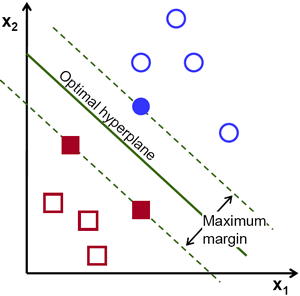
\includegraphics[width=0.5\textwidth]{svm}
\end{figure}
\end{frame}

\begin{frame}{Results: SVM Classification}

\textbf{One v/s One}:
\large
\begin{columns}
  \begin{column}{0.5\textwidth}
% Please add the following required packages to your document preamble:
% \usepackage{multirow}
\begin{table}[]
\centering
\begin{tabular}{l|l|l|l|}
\cline{2-4}
                                                                  & \multicolumn{3}{l|}{\textbf{Ground Truth}} \\ \hline
\multicolumn{1}{|l|}{\multirow{3}{*}{\rotatebox{90}{\textbf{Predict}}}} & 8         & 0         & 0        \\ \cline{2-4} 
\multicolumn{1}{|l|}{}                                            & 2          & 10         & 6        \\ \cline{2-4} 
\multicolumn{1}{|l|}{}                                            & 0          & 0         & 4        \\ \hline
\end{tabular}
\caption{C=16, $\sigma$ 16}
\label{my-label}
\end{table}
  \vspace{-20pt}
  \centering CCR: 73.33\%
  \end{column}
  \begin{column}{0.5\textwidth}  %%<--- here
% Please add the following required packages to your document preamble:
% \usepackage{multirow}
\begin{table}[]
\centering
\begin{tabular}{l|l|l|l|}
\cline{2-4}
                                                                  & \multicolumn{3}{l|}{\textbf{Ground Truth}} \\ \hline
\multicolumn{1}{|l|}{\multirow{3}{*}{\rotatebox{90}{\textbf{Predict}}}} & 10        & 0         & 0         \\ \cline{2-4} 
\multicolumn{1}{|l|}{}                                            & 0        & 9        & 2         \\ \cline{2-4} 
\multicolumn{1}{|l|}{}                                            & 0         & 1         & 8        \\ \hline
\end{tabular}
\caption{C=16, $\sigma$ 32}
\label{my-label}
\end{table}
  \vspace{-20pt}
  \centering CCR: 90\%
  \end{column}
\end{columns}
\end{frame}


\begin{frame}{Results: SVM Classification}
\textbf{One v/s All}:
\begin{itemize}
\item Mean CCR = 71.11\% (C = 2, $\sigma$ = 16)
\item Mean CCR = 88.9\% (C = 2, $\sigma$ = 32)
\end{itemize}
\begin{table}[]
\centering
\begin{tabular}{l|l|l|l|l|l|l|l|l|}
\cline{2-3} \cline{5-6} \cline{8-9}
C1                                       & \multicolumn{2}{l|}{Ground Truth} & C2               & \multicolumn{2}{l|}{Ground Truth} & C3               & \multicolumn{2}{l|}{Ground Truth} \\ \hline
\multicolumn{1}{|l|}{\multirow{2}{*}{\rotatebox{90}{\textbf{Predict}}}} & 8               & 0               & \multirow{2}{*}{\rotatebox{90}{\textbf{Predict}}} & 7               & 1               & \multirow{2}{*}{\rotatebox{90}{\textbf{Predict}}} & 6               & 0               \\ \cline{2-3} \cline{5-6} \cline{8-9} 
\multicolumn{1}{|l|}{}                         & 2               & 20              &                          & 3               & 19              &                          & 4               & 20              \\ \hline
\end{tabular}
\caption{OVO (C = 2, $\sigma$ = 32)}
\label{my-label}
\end{table}
\end{frame}

{
\begin{frame}[standout]
  \Huge Thank You
\end{frame}
}

\appendix

\begin{frame}[allowframebreaks]{References}
	\tiny
  \bibliography{demo}
  \bibliographystyle{abbrv}

\end{frame}





\end{document}
